\documentclass[11pt,letterpaper]{article}
\usepackage[T1]{fontenc}
\usepackage[utf8]{inputenc}
\usepackage{lmodern}
\usepackage[margin=1in,headheight=15pt]{geometry}
\usepackage{amsmath,amssymb,amsthm,mathtools}
\usepackage{microtype,booktabs,array,enumitem,graphicx}
\usepackage{xcolor,tikz}
\usetikzlibrary{arrows.meta,positioning,calc}
\usepackage{fancyhdr}
\usepackage[colorlinks=true,linkcolor=blue!45!black,citecolor=blue!45!black,urlcolor=blue!45!black]{hyperref}
\usepackage[nameinlink,noabbrev]{cleveref}
\hypersetup{pdftitle={Bridge Shear and Vortex Positivity for the Riemann Xi Function},pdfauthor={Jude Gomila},pdfsubject={Exact identities and a conditional route to the Riemann hypothesis}}
\pagestyle{fancy}
\fancyhf{}
\fancyhead[L]{\small Bridge shear and vortex positivity}
\fancyhead[R]{\small Research draft}
\fancyfoot[C]{\thepage}
\renewcommand{\headrulewidth}{0.3pt}
\setlength{\parskip}{0.35em}
\setlength{\parindent}{1.1em}
\setlist[itemize]{topsep=3pt,itemsep=3pt,leftmargin=1.5em}
\setlist[enumerate]{topsep=3pt,itemsep=3pt,leftmargin=2em}
\allowdisplaybreaks[2]
\numberwithin{equation}{section}
\newtheorem{theorem}{Theorem}[section]
\newtheorem{proposition}[theorem]{Proposition}
\newtheorem{lemma}[theorem]{Lemma}
\newtheorem{corollary}[theorem]{Corollary}
\theoremstyle{definition}
\newtheorem{definition}[theorem]{Definition}
\newtheorem{problem}[theorem]{Open problem}
\theoremstyle{remark}
\newtheorem{remark}[theorem]{Remark}
\newcommand{\R}{\mathbb R}
\newcommand{\C}{\mathbb C}
\newcommand{\Cp}{\mathbb C_+}
\newcommand{\dd}{\,\mathrm d}
\newcommand{\RH}{\mathrm{RH}}
\newcommand{\Repart}{\operatorname{Re}}
\newcommand{\Impart}{\operatorname{Im}}
\newcommand{\calC}{\mathcal C}
\newcommand{\calM}{\mathcal M}
\newcommand{\sh}{\mathrm{sh}}
\newcommand{\repo}{\href{https://github.com/judegomila/mathexplorer/tree/942ba1760c4ef54a519750ab91c37a661c31e0ce}{\texttt{mathexplorer}, commit \texttt{942ba1760c4e}}}

\title{\textbf{Bridge Shear and Vortex Positivity\\for the Riemann Xi Function}\\[0.5em]\large Exact identities and a conditional route to the Riemann hypothesis}
\author{Jude Gomila\\[0.2em]\small Research draft prepared with mathematical and editorial AI assistance}
\date{2 November 2026}

\begin{document}
\maketitle
\begin{abstract}
We study the shifted pair $E_a(z)=\Xi(z+ia)=A_a(z)-iB_a(z)$ used in the Zeta Explorer bridge construction, where $\Xi(z)=\xi(1/2+iz)$. Its scalar shear $W_a=A_aB_a'-A_a'B_a$ is simultaneously a component of the weighted phase current, one half of the transverse derivative of $|\Xi|^2$, and the real diagonal of a shifted de Branges kernel. We derive a complex-diagonal averaging identity and an explicit negative kernel witness associated with any hypothetical nonreal zero of $\Xi$. We then express the complete shear as the Fourier transform of a positive theta-interaction profile; positive definiteness of that profile is equivalent to the required global sign. Theta modularity gives cancellation of all odd endpoint derivatives. Nevertheless, every naive finite theta-index truncation has eventually negative shear, with leading term $-2a[\psi_N'(0)]^2t^{-6}$. We connect the full profile to generalized Laguerre inequalities, describe exact Schur-complement closure conditions, and explain the limits of spherical compactification. The global positive-definiteness assertion remains unproved. This paper supplies exact reductions and obstruction results, not a proof of the Riemann hypothesis.
\end{abstract}

\section{Scope and logical status}
The motivating question is whether the phase vortices of zeta, linked by a reflection-symmetric bridge and displayed on a Riemann sphere, can force all nontrivial zeros onto the critical line. The appropriate analytic object is the completed function $\xi$, whose zeros are exactly the nontrivial zeros of $\zeta$. A useful direction field is obtained from its phase; an even more convenient quantity multiplies that field by $|\xi|^2$, removing the local singularity at each zero.

We use the exact shifted functions and kernel in \repo\ \cite{repo}. The repaired paired-coordinate derivation in that repository is the starting point. In particular, we do not use a nonzero contribution attributed to the diagonal of a two-dimensional Lebesgue integral, nor assert that the bare antisymmetric shear operator is positive. Both assertions would be invalid.

The paper has three types of statement. The analytic identities and endpoint obstruction below are proved directly. The equivalences with RH are conditional reductions: they establish what a successful positivity theorem would imply. The missing positive-definiteness statement is explicitly designated an open problem. No finite calculation or spherical index argument is used to cross that gap.

\paragraph{Relation to prior work.}
Positivity of $\Repart(\xi'/\xi)$ is an established RH criterion, treated by Lagarias \cite{lagarias,lagariasCorrection}; horizontal monotonicity is discussed by Sondow and Dumitrescu \cite{sondow}. Shifted quotients, inner functions and associated canonical systems are studied by Suzuki \cite{suzuki}. Generalized Laguerre inequalities and positive definite associated kernels are treated by Csordas--Vishnyakova \cite{cv}, Cardon \cite{cardon}, and Csordas \cite{csordas}. Planat gives a closely related theta-kernel growth reformulation and discusses obstruction to phase-aligned blockwise positivity \cite{planat,planatCompanion}. We do not claim novelty for the positivity criteria, the paired theta structure, or their general relation to RH. The present purpose is to put the actual Explorer shear, its vortex interpretation, its exact normalization and its truncation obstruction into one auditable argument. The finite theta-index obstruction proved here is distinct from a statement about phase-aligned integration blocks; no priority claim is made for it.

\paragraph{How to read the argument.}
Sections 2--4 establish the functions, vortex identity and zero witness. Sections 5--7 retain the complete theta interaction, prove the modular cancellations and quantify the failure of finite truncation. Sections 8--9 formulate two all-level positivity routes. Sections 10--11 treat the sphere and the exact remaining proof obligation. Figure~\ref{fig:route} records the gap explicitly.

\begin{figure}[p]
\centering
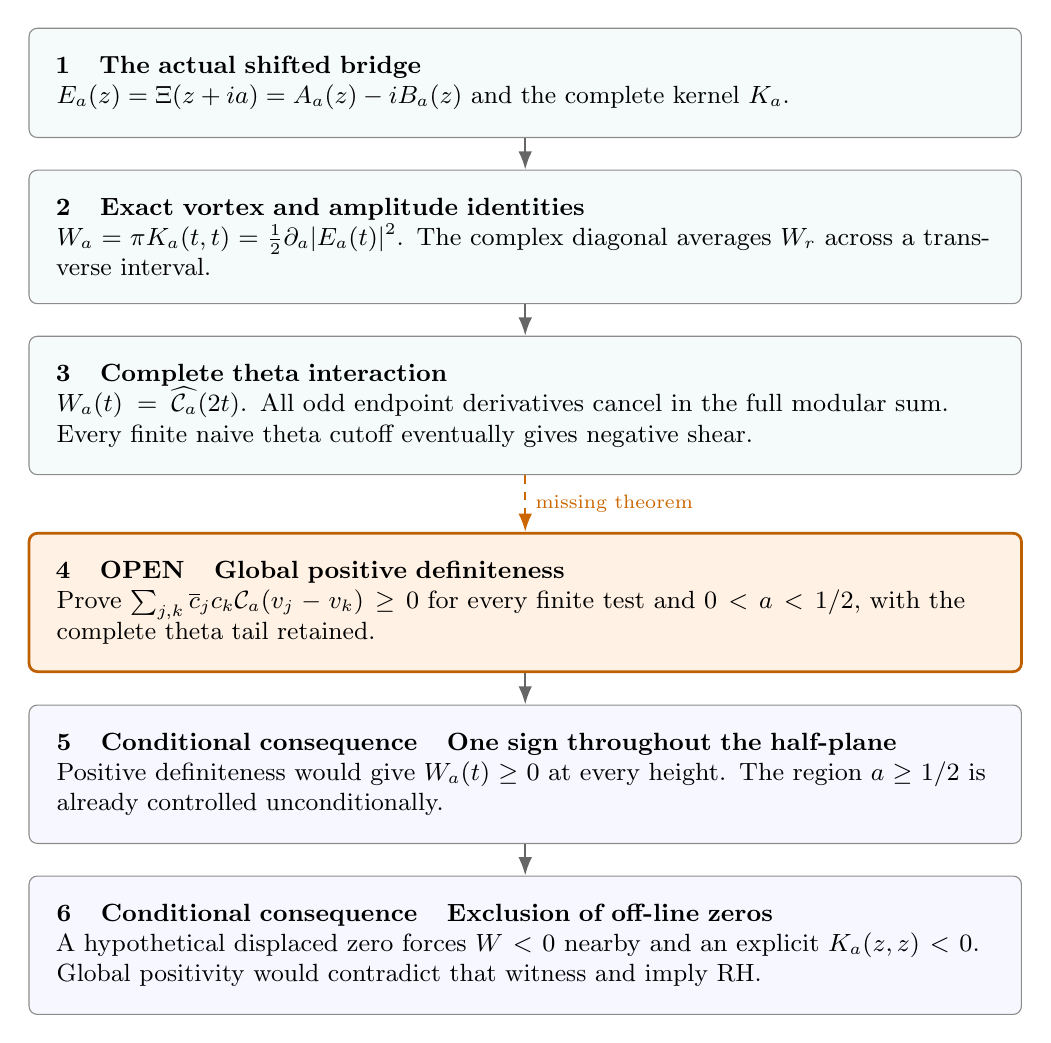
\begin{tikzpicture}[node distance=0.40cm,>=Latex,
  routebox/.style={draw=black!45,rounded corners=3pt,text width=11.9cm,align=left,inner sep=10pt,font=\small},
  established/.style={routebox,fill=teal!4},
  unresolved/.style={routebox,draw=orange!75!black,fill=orange!10,line width=1pt},
  conditional/.style={routebox,fill=blue!3},
  flow/.style={->,thick,draw=black!60}]
\node[established] (a) {\textbf{1\quad The actual shifted bridge}\par $E_a(z)=\Xi(z+ia)=A_a(z)-iB_a(z)$ and the complete kernel $K_a$.};
\node[established,below=of a] (b) {\textbf{2\quad Exact vortex and amplitude identities}\par $W_a=\pi K_a(t,t)=\tfrac12\partial_a|E_a(t)|^2$. The complex diagonal averages $W_r$ across a transverse interval.};
\node[established,below=of b] (c) {\textbf{3\quad Complete theta interaction}\par $W_a(t)=\widehat{\calC_a}(2t)$. All odd endpoint derivatives cancel in the full modular sum. Every finite naive theta cutoff eventually gives negative shear.};
\node[unresolved,below=0.72cm of c] (d) {\textbf{4\quad OPEN\quad Global positive definiteness}\par Prove $\sum_{j,k}\overline c_jc_k\calC_a(v_j-v_k)\ge0$ for every finite test and $0<a<1/2$, with the complete theta tail retained.};
\node[conditional,below=of d] (e) {\textbf{5\quad Conditional consequence\quad One sign throughout the half-plane}\par Positive definiteness would give $W_a(t)\ge0$ at every height. The region $a\ge1/2$ is already controlled unconditionally.};
\node[conditional,below=of e] (f) {\textbf{6\quad Conditional consequence\quad Exclusion of off-line zeros}\par A hypothetical displaced zero forces $W<0$ nearby and an explicit $K_a(z,z)<0$. Global positivity would contradict that witness and imply RH.};
\draw[flow] (a)--(b);
\draw[flow] (b)--(c);
\draw[flow,dashed,draw=orange!80!black] (c)-- node[right,font=\scriptsize,text=orange!80!black]{missing theorem} (d);
\draw[flow] (d)--(e);
\draw[flow] (e)--(f);
\end{tikzpicture}
\caption{The logical route. Steps 1--3 are established in this paper. The dashed transition is not a proved implication. Steps 5--6 are proved consequences of the open assertion in Step 4. The figure does not depict a completed proof of RH.}
\label{fig:route}
\end{figure}

\section{Functions and the modular theta profile}
\subsection{Conventions}
Throughout,
\begin{equation}\label{eq:xi}
\xi(s)=\tfrac12s(s-1)\pi^{-s/2}\Gamma(s/2)\zeta(s),\qquad
\Xi(z)=\xi(\tfrac12+iz).
\end{equation}
The function $\Xi$ is real entire, even, of order one, and satisfies $\Xi(0)\ne0$. Its zeros lie in $|\Impart z|<1/2$. RH is equivalent to the assertion that all of its zeros are real. We count zeros with multiplicity. These standard facts and the canonical products used below follow from the usual analytic continuation and functional equation of $\xi$ \cite{dlmf,lagarias}.

For $a\in\R$ define
\begin{equation}\label{eq:pair}
E_a(z)=\Xi(z+ia)=A_a(z)-iB_a(z),\qquad
E_a^\#(z):=\overline{E_a(\bar z)}=\Xi(z-ia),
\end{equation}
where
\begin{equation}\label{eq:AB}
A_a(z)=\frac{\Xi(z+ia)+\Xi(z-ia)}2,\qquad
B_a(z)=\frac{\Xi(z-ia)-\Xi(z+ia)}{2i}.
\end{equation}
Both $A_a$ and $B_a$ are real entire. A prime denotes differentiation in the spectral variable $z$, or in real $t$ when restricted to the real axis. Set
\begin{equation}\label{eq:HW}
H(a,t)=|E_a(t)|^2,\qquad
W_a(t)=A_a(t)B_a'(t)-A_a'(t)B_a(t).
\end{equation}
Then $H$ is even in $a$ and $W$ is odd in $a$.

\subsection{The exact theta normalization}
The Explorer convention is
\begin{align}
\Xi(z)&=8\int_0^\infty\Phi(u)\cos(2zu)\dd u,\label{eq:PhiTransform}\\
\Phi(u)&=\sum_{n=1}^\infty\phi_n(u),\qquad
\phi_n(u)=\bigl(2\pi^2n^4e^{9u}-3\pi n^2e^{5u}\bigr)e^{-\pi n^2e^{4u}}.\label{eq:Phi}
\end{align}
For the calculations it is convenient to use the equivalent profile
\begin{equation}\label{eq:psi}
\psi(v)=4\Phi(v/2),\qquad
\Xi(z)=\int_0^\infty\psi(v)\cos(zv)\dd v.
\end{equation}
This fixes all factors of two; no normalization from another theta convention is silently substituted.

\begin{lemma}[Modular evenness and endpoint identities]\label{lem:modularity}
The full profile $\Phi$ is smooth, even and strictly positive on $\R$. Its derivatives decay faster than every exponential as $u\to+\infty$. The series defining it can be differentiated termwise on compact real intervals, and
\begin{equation}\label{eq:oddjets}
\sum_{n\ge1}\phi_n^{(2k+1)}(0)=0,\qquad k=0,1,2,\ldots.
\end{equation}
The same smoothness, evenness and decay statements hold for $\psi$.
\end{lemma}
\begin{proof}
Let $\vartheta(x)=\sum_{n\in\mathbb Z}e^{-\pi n^2x}$ for $x>0$, and use the Jacobi identity $\vartheta(x)=x^{-1/2}\vartheta(1/x)$. The function
\[
g(u)=e^u\vartheta(e^{4u})
\]
is even. Direct differentiation of its locally uniformly convergent series gives
\[
g''(u)-g(u)=16\Phi(u).
\]
Thus $\Phi$ is even. On $u\ge0$, put $r=\pi n^2e^{4u}$; then $\phi_n(u)=e^ur(2r-3)e^{-r}>0$. Evenness gives positivity on the other half-line. On a compact real interval every differentiated summand is bounded by a polynomial in $n$ times $e^{-c n^2}$ for some $c>0$, which justifies termwise differentiation. On the positive half-line the factor $e^{-\pi n^2e^{4u}}$ gives the asserted decay, also after differentiation. Every odd derivative at the origin therefore vanishes, proving \eqref{eq:oddjets}.
\end{proof}

It follows that the integrals below, including their derivatives and fixed-$a$ exponential weights, converge absolutely. In particular,
\begin{equation}\label{eq:ABintegrals}
\begin{aligned}
A_a(z)&=\int_0^\infty\psi(u)\cosh(au)\cos(zu)\dd u,\\
B_a(z)&=\int_0^\infty\psi(u)\sinh(au)\sin(zu)\dd u.
\end{aligned}
\end{equation}

\section{The shear as a vortex current}
\begin{proposition}[Vortex and amplitude identity]\label{prop:vortex}
For real $a,t$,
\begin{equation}\label{eq:Widentity}
W_a(t)=\tfrac12\partial_aH(a,t)
=\Repart\!\left(\xi'(\tfrac12+a+it)\overline{\xi(\tfrac12+a+it)}\right).
\end{equation}
Away from zeros, this equals
\begin{equation}\label{eq:Wlog}
H(a,t)\Repart\frac{\xi'}{\xi}(\tfrac12+a+it)
=H(a,t)\partial_t\arg\xi(\tfrac12+a+it).
\end{equation}
\end{proposition}
\begin{proof}
The functional equation and conjugation give $F(a,t):=\xi(1/2+a+it)=\overline{E_a(t)}=A_a(t)+iB_a(t)$. As a function of $a+it$, $F$ is holomorphic, so $\partial_a A=\partial_t B$ and $\partial_a B=-\partial_t A$. Hence
\[
\tfrac12\partial_a(A^2+B^2)=AB'-A'B=W_a.
\]
The last expression in \eqref{eq:Widentity} follows by differentiating $|F|^2$. Dividing by $H$ away from zeros, and differentiating the argument, proves \eqref{eq:Wlog}. The undivided identity is valid at zeros as well.
\end{proof}

If $\xi'/\xi=u+iv$, the weighted phase current in coordinates $(a,t)$ is
\begin{equation}\label{eq:current}
j=H\nabla\arg F=(Hv,W_a).
\end{equation}
A clockwise rotation through $\pi/2$ gives
\[
R_{-\pi/2}j=(W_a,-Hv)=\tfrac12\nabla H.
\]
Thus $W_a$ measures both a tangential component of phase flow and an outward component of the amplitude-gradient current. This is a directional statement. It does not assert that phase trajectories dynamically move the zeros or that every trajectory converges to the critical line.

\begin{lemma}[A local negative witness]\label{lem:localnegative}
Suppose $\xi$ has a zero $\rho=1/2+a_0+i\gamma$ with $a_0>0$ and multiplicity $m$. Then $W_{a_0-\varepsilon}(\gamma)<0$ for all sufficiently small $\varepsilon>0$.
\end{lemma}
\begin{proof}
Write $\xi(s)=c(s-\rho)^m+O((s-\rho)^{m+1})$ with $c\ne0$. On the horizontal line through $\rho$,
\[
W_{a_0-\varepsilon}(\gamma)
=-m|c|^2\varepsilon^{2m-1}+O(\varepsilon^{2m}).
\]
The leading coefficient is negative. Equivalently, $\xi'/\xi=-m/\varepsilon+O(1)$ there. The analytic factor containing all other zeros cannot remove this local sign.
\end{proof}

\begin{theorem}[Global scalar criterion]\label{thm:scalar}
The following are equivalent:
\begin{enumerate}[label=(\roman*)]
\item RH;
\item $W_a(t)\ge0$ for every $a>0$ and $t\in\R$;
\item $a\mapsto H(a,t)$ is nondecreasing on $[0,\infty)$ for every $t\in\R$.
\end{enumerate}
Under RH, $W_a(t)>0$ for every $a>0,t\in\R$.
\end{theorem}
\begin{proof}
Under RH the centered canonical product gives
\begin{equation}\label{eq:Poisson}
\Repart\frac{\xi'}{\xi}(\tfrac12+a+it)
=\sum_{\gamma\in\R}\frac{m_\gamma a}{a^2+(t-\gamma)^2}>0.
\end{equation}
The sum converges locally absolutely for $a>0$; the usual zero count implies $\sum_{\gamma\ne0}m_\gamma/\gamma^2<\infty$. There is no zero in this half-plane under RH, so \cref{prop:vortex} proves (ii), with strict positivity. Conversely, (ii) excludes every right-hand off-line zero by \cref{lem:localnegative}; the functional equation excludes its reflected left-hand partner. Finally, (ii) and (iii) are equivalent by \eqref{eq:Widentity}. An alternative proof of (iii)$\Rightarrow$(i) is that a nonnegative nondecreasing $H(a,t_0)$ could not vanish at $a_0>0$ unless it vanished throughout $0\le a\le a_0$, forcing an entire function to vanish identically.
\end{proof}

\subsection{What reflected vortices cancel}
Put $\mathcal F(z)=\xi(1/2+z)$. A reflected pair of centered zeros $\pm b+i\gamma$, of the same multiplicity $m$, contributes
\begin{equation}\label{eq:pairfield}
q_{b,\gamma}(z)=\frac{m}{z-b-i\gamma}+\frac{m}{z+b-i\gamma}.
\end{equation}
Writing $u=z-i\gamma$ gives the convergent expansion
\begin{equation}\label{eq:multipole}
q_{b,\gamma}(z)=\frac{2m}{u}+\frac{2mb^2}{u^3}+\frac{2mb^4}{u^5}+\cdots,
\qquad |u|>|b|.
\end{equation}
Odd transverse moments cancel. The leading term resembles two coincident line vortices, but every even displacement moment remains. Direct algebra yields, for $x>0$ and away from the pair,
\begin{equation}\label{eq:pairSign}
\Repart q_{b,\gamma}(x+it)=
\frac{2mx\{x^2+(t-\gamma)^2-b^2\}}
{\{(x-b)^2+(t-\gamma)^2\}\{(x+b)^2+(t-\gamma)^2\}}.
\end{equation}
Thus a negative contribution is possible only when $0<x<|b|$ and $|t-\gamma|<\sqrt{b^2-x^2}$. A zero on the line contributes $mx/(x^2+(t-\gamma)^2)>0$ and is counted once, rather than twice as an artificially duplicated pair.

Pairing centered zeros $\alpha$ and $-\alpha$ in the even order-one Hadamard product removes a residual linear exponential factor. Taking real parts gives
\begin{equation}\label{eq:unconditionalZeroSum}
\Repart\frac{\mathcal F'}{\mathcal F}(x+it)
=\sum_{\alpha=b+i\gamma}\frac{x-b}{(x-b)^2+(t-\gamma)^2},
\end{equation}
with multiplicities. This real-part sum is locally absolutely convergent away from zeros, since $|b|<1/2$ and the terms at large $|\gamma|$ are $O(\gamma^{-2})$ on compact sets. It can therefore be regrouped into the reflected pairs in \eqref{eq:pairSign}. That formula proves unconditional positivity for $x\ge1/2$. At a fixed point, every reflected pair with $|t-\gamma|\ge1/2$ contributes nonnegatively. Only finitely many nearby heights can contribute negatively. This localizes the unknown transverse region to $0<x<1/2$; it does not determine the unknown zero locations or establish the sign there.

\section{The complete shifted kernel and a zero exclusion theorem}
Define the Hermitian kernel on $\Cp=\{z:\Impart z>0\}$ by
\begin{equation}\label{eq:K}
\begin{aligned}
K_a(w,z)
&=\frac{\overline{A_a(w)}B_a(z)-\overline{B_a(w)}A_a(z)}{\pi(z-\bar w)}\\
&=\frac{\overline{E_a(w)}E_a(z)-\overline{E_a^\#(w)}E_a^\#(z)}{2\pi i(\bar w-z)}.
\end{aligned}
\end{equation}
On real nodes use removable continuation. Then $K_a(t,t)=W_a(t)/\pi$.

\begin{proposition}[The complex diagonal averages the vortex shear]\label{prop:average}
For $a,y>0$ and real $t$,
\begin{equation}\label{eq:average}
K_a(t+iy,t+iy)
=\frac{H(a+y,t)-H(a-y,t)}{4\pi y}
=\frac1{2\pi y}\int_{|a-y|}^{a+y}W_r(t)\dd r.
\end{equation}
In particular,
\begin{equation}\label{eq:limitcomplex}
\lim_{a\downarrow0}\frac{K_a(t+iy,t+iy)}a
=\frac{W_y(t)}{\pi y}.
\end{equation}
\end{proposition}
\begin{proof}
In the second expression of \eqref{eq:K}, the denominator at $z=w=t+iy$ is $4\pi y$. The squared moduli in the numerator are $H(y+a,t)$ and $H(y-a,t)$. Use evenness of $H$, then integrate $\partial_rH=2W_r$. Differentiation at $a=0$ gives \eqref{eq:limitcomplex}. All these operations concern smooth entire quantities, so no division by $\Xi$ is involved.
\end{proof}

\begin{proposition}[An explicit negative bridge diagonal]\label{prop:kernelwitness}
If $\Xi(\lambda_0)=0$ and $b=\Impart\lambda_0>0$, then for all sufficiently small $a>0$, with $a<b$, the point $z_0=\lambda_0-ia$ satisfies
\begin{equation}\label{eq:kernelwitness}
K_a(z_0,z_0)
=-\frac{|\Xi(\lambda_0-2ia)|^2}{4\pi(b-a)}<0.
\end{equation}
\end{proposition}
\begin{proof}
Isolation of $\lambda_0$ gives a disk containing no distinct zero. For sufficiently small nonzero $a$, $\lambda_0-2ia$ lies in that disk and is not a zero. But $E_a(z_0)=\Xi(\lambda_0)=0$, while $E_a^\#(z_0)=\Xi(\lambda_0-2ia)\ne0$. Substitute in \eqref{eq:K}. The proof works for arbitrary multiplicity and avoids a possible common-zero degeneracy at a fixed larger shift.
\end{proof}

\begin{theorem}[Small-shift complex-diagonal criterion]\label{thm:sequence}
Fix any positive sequence $a_j\to0$. The following are equivalent:
\begin{enumerate}[label=(\roman*)]
\item RH;
\item $K_{a_j}(z,z)\ge0$ for all $j$ and all $z\in\Cp$;
\item every finite Gram matrix $[K_{a_j}(z_k,z_\ell)]_{k,\ell=1}^N$ is positive semidefinite, for all $j$ and all finite node sets in $\Cp$.
\end{enumerate}
\end{theorem}
\begin{proof}
Condition (iii) implies (ii). Condition (ii) implies $W_y(t)\ge0$ by dividing by $a_j$ and using \eqref{eq:limitcomplex}, so \cref{thm:scalar} gives RH. Alternatively \cref{prop:kernelwitness} contradicts (ii) directly if a nonreal zero exists.

For (i)$\Rightarrow$(iii), approximate $\Xi$ by the locally uniformly convergent real-rooted product polynomials
\[
P_N(z)=\Xi(0)\prod_{0<\gamma\le T_N}(1-z^2/\gamma^2)^{m_\gamma}.
\]
For a real root $r$, the shifted quotient $b_r(z)=(z-r-ia)/(z-r+ia)$ has kernel
\[
\frac{1-\overline{b_r(w)}b_r(z)}{2\pi i(\bar w-z)}
=\frac{a}{\pi(\bar w-r-ia)(z-r+ia)},
\]
which is a positive rank-one kernel. The identity
\[
1-\overline{UV(w)}UV(z)
=[1-\overline{U(w)}U(z)]
+\overline{U(w)}U(z)[1-\overline{V(w)}V(z)]
\]
shows by induction that every finite product quotient has a positive kernel. Multiplying by $\overline{P_N(w+ia)}P_N(z+ia)$ preserves positivity and gives the kernel associated with $P_N$. Local uniform convergence passes every finite Gram inequality to $K_a$. This proves (iii), for every $a>0$.
\end{proof}

\begin{remark}
Positivity of an arbitrary kernel on its diagonal does not imply positive definiteness. The equivalence above is special to the complete family built from $\Xi$, and its proof passes through RH. Positivity of only the \emph{real diagonal} $K_{a_j}(t,t)$, even for every real $t$ and a sequence $a_j\to0$, does not give \cref{thm:sequence}; the variable $y>0$ in \eqref{eq:limitcomplex} is essential to that diagonal criterion. This limitation concerns scalar diagonal tests, not all finite real-node Gram matrices. Section~\ref{sec:Laguerre} and Appendix~\ref{app:counterexample} give explicit counterexamples to the diagonal-only shortcut.
\end{remark}

\section{The paired shear and its scalar interaction profile}
\subsection{Retaining the complete two-variable kernel}
Put
\[
r=(u+v)/2,\qquad s=(v-u)/2,\qquad
M(r,s)=\psi(r-s)\psi(r+s),
\]
and $\Delta=\bar w-z$, $\Sigma=\bar w+z$. The complete paired representation is
\begin{equation}\label{eq:pairedK}
\begin{split}
K_a(w,z)=\frac2\pi\int_0^\infty\!\int_0^r M(r,s)
\bigg[&\sinh(2ar)\frac{\sin(\Delta r)}{\Delta}\cos(\Sigma s)\\
&+\sinh(2as)\frac{\sin(\Delta s)}{\Delta}\cos(\Sigma r)\bigg]\dd s\dd r.
\end{split}
\end{equation}
The sine quotient has its continuous value at $\Delta=0$. To verify the formula, insert \eqref{eq:ABintegrals} into \eqref{eq:K}, interchange the absolutely convergent integrals, set $(u,v)=(r-s,r+s)$, and pair $s$ with $-s$. The Jacobian is $2$; the product-to-sum identities leave the two terms displayed in \eqref{eq:pairedK}. This is the repaired identity in the repository audit \cite{repo}.

On the real diagonal it gives
\begin{equation}\label{eq:pairedW}
\begin{split}
W_a(t)=2\int_0^\infty\!\int_0^r M(r,s)
\big[&r\sinh(2ar)\cos(2ts)\\
&+s\sinh(2as)\cos(2tr)\big]\dd s\dd r.
\end{split}
\end{equation}
Neither oscillatory channel in this identity can be discarded when estimating the full sign.

\begin{remark}[Two invalid positivity shortcuts]\label{rem:invalid}
The set $u=v$ has two-dimensional Lebesgue measure zero. A one-dimensional positive expression obtained by evaluating the integrand there is a comparison object, not a nonzero summand of the original double integral. An add-and-subtract comparison requires a bound for the complete resulting remainder.

Also, the raw shear $g_a(u,v)=\psi(u)\psi(v)\sinh(a(v-u))$ equals $p(u)q(v)-q(u)p(v)$, with $p=\psi\cosh(a\cdot)$ and $q=\psi\sinh(a\cdot)$. On $L^2(0,\infty)$ it is skew-adjoint and has rank at most two. Unless it vanishes, $ig_a$ has one positive and one negative eigenvalue, namely
\[
\pm\sqrt{\|p\|^2\|q\|^2-|\langle p,q\rangle|^2}.
\]
The desired positive object is the complete transformed kernel, not this raw operator.
\end{remark}

\subsection{A complete scalar profile}
\begin{definition}\label{def:C}
For $a>0$ and $v\in\R$, use the full even profile $\psi$ and set
\begin{equation}\label{eq:C}
\calC_a(v)=\int_0^\infty h\sinh(2ah)\psi(h-v)\psi(h+v)\dd h.
\end{equation}
Our notation $\calC_a$ does not denote the implementation's normalized component $B_a/a$.
\end{definition}

\begin{proposition}[Exact Fourier representation]\label{prop:Cfourier}
The function $\calC_a$ is even, smooth, strictly positive and rapidly decaying together with all its derivatives. With $\widehat f(k)=\int_\R f(v)e^{-ikv}\dd v$,
\begin{equation}\label{eq:WFourier}
W_a(t)=2\int_0^\infty\calC_a(v)\cos(2tv)\dd v
=\widehat{\calC_a}(2t).
\end{equation}
\end{proposition}
\begin{proof}
In the first term of \eqref{eq:pairedW}, fix $s=v$ and integrate $r=h$ from $v$ to infinity. In the second term, fix $r=v$ and integrate $s=h$ from zero to $v$. The two inner integrals combine into
\[
\int_0^\infty h\sinh(2ah)\psi(|h-v|)\psi(h+v)\dd h.
\]
Evenness of $\psi$ gives \eqref{eq:C}; evenness of $\calC_a$ then gives \eqref{eq:WFourier}. Positivity follows from the positive integrand. Smoothness uses the smooth even extension, rather than differentiating a cusp. For the decay, note that $\max(|h-v|,|h+v|)=h+|v|$ for $h\ge0$. One of the two differentiated profiles therefore supplies super-exponential decay in $h+|v|$, dominating the fixed weight $h\sinh(2ah)$ and every polynomial. Differentiation under the integral and all asserted rapid-decay bounds follow.
\end{proof}

\begin{definition}
A continuous function $C:\R\to\C$ is positive definite if
\begin{equation}\label{eq:PD}
\sum_{j,k=1}^N\overline{c_j}c_k C(v_j-v_k)\ge0
\end{equation}
for every $N$, real $v_1,\ldots,v_N$, and complex $c_1,\ldots,c_N$. The convention permits positive semidefinite, rather than strictly positive, matrices.
\end{definition}

\begin{theorem}[The scalar theta positivity target]\label{thm:Ccriterion}
For each fixed $a>0$,
\[
W_a(t)\ge0\text{ for all }t\in\R
\quad\Longleftrightarrow\quad
\calC_a\text{ is positive definite}.
\]
Consequently RH is equivalent to positive definiteness of $\calC_a$ for every $a>0$. It suffices to establish this for $0<a<1/2$.
\end{theorem}
\begin{proof}
For a Schwartz function, positive definiteness is equivalent to a nonnegative Fourier transform. In one direction, Fourier inversion gives
\[
\sum_{j,k}\overline{c_j}c_kC(v_j-v_k)
=\frac1{2\pi}\int_\R\widehat C(k)
\left|\sum_jc_je^{-ikv_j}\right|^2\dd k\ge0.
\]
Conversely, finite positive forms imply the analogous integral quadratic forms by approximation with Riemann sums; Fourier localization at a point where the continuous $\widehat C$ were negative would contradict those forms. Apply this equivalence to \cref{prop:Cfourier}, then use \cref{thm:scalar}. The last assertion follows from the unconditional region $a\ge1/2$ established using \eqref{eq:pairSign}.
\end{proof}

Pointwise positivity of \eqref{eq:C} is not positive definiteness. The latter is an assertion about every coupled test \eqref{eq:PD}. This is the precise additional statement needed to turn the full theta interaction into the global vortex sign.

\section{Modular cancellation at every algebraic order}\label{sec:cancellation}
\begin{proposition}[Complete endpoint cancellation]\label{prop:rapid}
For each fixed $a>0$ and each positive integer $L$,
\begin{equation}\label{eq:rapid}
W_a(t)=O_{a,L}((1+|t|)^{-L}).
\end{equation}
In the half-line cosine expansion of \eqref{eq:WFourier}, every algebraic endpoint coefficient vanishes.
\end{proposition}
\begin{proof}
The full $\calC_a$ is an even Schwartz function by \cref{prop:Cfourier}, so its Fourier transform is Schwartz. Equivalently, repeated integration by parts in the half-line cosine transform gives endpoint coefficients proportional to the odd derivatives $\calC_a^{(2k+1)}(0)$; these all vanish because $\calC_a$ is smooth and even. The full smooth extension ultimately uses \cref{lem:modularity}.
\end{proof}

The two individual sectors of \eqref{eq:pairedW} generally retain algebraic terms. Let $S_a$ be the second, sum-frequency sector, and $D_a$ the first sector. Then
\begin{equation}\label{eq:sectors}
S_a(t)=\frac{a\psi(0)^2}{2t^4}+O_a(t^{-6}),\qquad
D_a(t)=-\frac{a\psi(0)^2}{2t^4}+O_a(t^{-6}).
\end{equation}
Indeed, the inner integral in $S_a$ satisfies
\[
\int_0^r\psi(r-s)\psi(r+s)s\sinh(2as)\dd s
=\frac{2a\psi(0)^2}{3}r^3+O_a(r^5).
\]
Including the outer factor $2$ and integrating the cosine transform by parts gives the first asymptotic in \eqref{eq:sectors}. Since $D_a+S_a=W_a$ is rapidly decreasing, the second follows. Complete endpoint expansions, when taken to any fixed algebraic order, cancel between the two sectors.

These are exact cancellation statements. They do not decide whether the remaining $W_a(t)$ is positive, negative or zero at a given point. In particular, a remainder smaller than every inverse power can have either sign. Related cancellation obstructions for a different phase-aligned block decomposition are discussed in \cite{planat,planatCompanion}; those results are not used as premises here.

\section{The obstruction to ordinary finite theta truncation}
Define the ordinary half-line cutoff
\begin{equation}\label{eq:psiN}
\psi_N(v)=4\sum_{n=1}^N\phi_n(v/2),\qquad v\ge0,
\end{equation}
and form $A_{a,N},B_{a,N}$ by replacing $\psi$ with $\psi_N$ in \eqref{eq:ABintegrals}. This is a specific truncation; the theorem below does not concern every possible approximation scheme.

\begin{lemma}[Every finite cutoff has a nonzero endpoint defect]\label{lem:dN}
For every integer $N\ge1$, $d_N:=\psi_N'(0)>0$.
\end{lemma}
\begin{proof}
With $r_n=\pi n^2$, direct differentiation gives
\begin{equation}\label{eq:phiDerivative}
\phi_n'(0)=e^{-r_n}r_n(-8r_n^2+30r_n-15).
\end{equation}
The quadratic $g(r)=-8r^2+30r-15$ decreases for $r>15/8$. Since $\pi<22/7$, $g(\pi)>g(22/7)=13/49>0$, so the $n=1$ derivative is positive. For $n\ge2$, $r_n>12$, and $g(r_n)<0$. By \cref{lem:modularity}, the convergent full derivative sum is zero. Therefore
\begin{equation}\label{eq:dN}
d_N=2\sum_{n\le N}\phi_n'(0)
=-2\sum_{n>N}\phi_n'(0)>0.
\end{equation}
\end{proof}

\begin{theorem}[Eventually negative finite-cutoff shear]\label{thm:cutoff}
For each fixed $N\ge1$ and each fixed $a>0$, the actual truncated shear satisfies
\begin{equation}\label{eq:negativeTail}
W_{a,N}(t)
=-\frac{2ad_N^2}{t^6}+O_{a,N}(t^{-8})
\qquad (|t|\to\infty).
\end{equation}
In particular $W_{a,N}(t)<0$ for all sufficiently large $|t|$.
\end{theorem}
\begin{proof}
All derivatives of the finite profile decay super-exponentially on the positive half-line. Put $f(v)=\psi_N(v)\cosh(av)$ and $g(v)=\psi_N(v)\sinh(av)$. Repeated integration by parts gives
\begin{align*}
A_{a,N}(t)&=-f'(0)t^{-2}+O_{a,N}(t^{-4})
=-d_Nt^{-2}+O_{a,N}(t^{-4}),\\
B_{a,N}(t)&=g(0)t^{-1}-g''(0)t^{-3}+O_{a,N}(t^{-5})
=-2ad_Nt^{-3}+O_{a,N}(t^{-5}).
\end{align*}
The differentiated integral representations, treated by the same integrations by parts, give
\[
A_{a,N}'(t)=2d_Nt^{-3}+O_{a,N}(t^{-5}),\qquad
B_{a,N}'(t)=6ad_Nt^{-4}+O_{a,N}(t^{-6}).
\]
Thus $AB'-A'B=(-6+4)ad_N^2t^{-6}+O_{a,N}(t^{-8})$, proving \eqref{eq:negativeTail}. We have not differentiated an uncontrolled big-$O$ term; the derivative estimates come from the differentiated integrals. Finally use $d_N>0$.
\end{proof}

\begin{remark}[Order of limits and scope]
The constants and the onset of negativity depend on $a$ and $N$. No uniform onset as $a\downarrow0$ or $N\to\infty$ is claimed. For each finite $N$, the endpoint defect is nonzero, although it becomes very small. Taking the full modular sum restores all odd-derivative identities. The result does not refute the full bridge, and does not invalidate a finite-window enclosure that includes a rigorous tail. It rules out treating the ordinary finite cutoff itself as an everywhere-positive global approximation.
\end{remark}

For orientation only, direct floating-point evaluation of the rapidly convergent tail in \eqref{eq:dN} gives the values below. Their signs are proved above; these decimal values are not interval certificates.
\begin{center}
\begin{tabular}{rcc}
\toprule
$N$ & $d_N$ & Leading coefficient $-d_N^2$ at $a=1/2$\\
\midrule
1 & $7.89975305355\times10^{-2}$ & $-6.24060983071\times10^{-3}$\\
2 & $1.65305591555\times10^{-7}$ & $-2.73259385992\times10^{-14}$\\
3 & $2.78345172722\times10^{-16}$ & $-7.74760351776\times10^{-32}$\\
\bottomrule
\end{tabular}
\end{center}

\begin{proposition}[A residual odd endpoint derivative forces a negative tail]\label{prop:generaljet}
Let $\psi$ be a real-valued smooth half-line profile such that $v^k e^{Av}\psi^{(j)}(v)\in L^1(0,\infty)$ for every $A>0$ and all nonnegative integers $j,k$. Suppose its first nonzero odd derivative at zero is $\psi^{(2m+1)}(0)=d\ne0$. For fixed $a>0$, its shear has the asymptotic
\begin{equation}\label{eq:generaljet}
W_a(t)=-(2m+2)ad^2t^{-(4m+6)}+O_a(t^{-(4m+8)}).
\end{equation}
\end{proposition}
\begin{proof}
Put $p=2m+2$ and $c=(-1)^{m+1}d$. The first nonvanishing endpoint coefficients in the cosine and sine transforms give $A=c t^{-p}+O(t^{-p-2})$ and $B=pa c t^{-p-1}+O(t^{-p-3})$. Applying the same argument to the differentiated integrals gives $AB'-A'B=-pa c^2t^{-2p-2}+O(t^{-2p-4})$. This is \eqref{eq:generaljet}.
\end{proof}

For a repair that leaves some odd endpoint derivative nonzero, this proposition shows that canceling earlier endpoint terms moves the negative tail to higher order without removing it. A structural operation that enforces full evenness, or a modularity-preserving approximation with a certified remainder, is not excluded.

\section{The all-orders Laguerre hierarchy}\label{sec:Laguerre}
For a nonzero real entire function $f$, define
\begin{equation}\label{eq:Ln}
L_n[f](t)=\sum_{j=0}^{2n}
\frac{(-1)^{j+n}}{j!(2n-j)!}f^{(j)}(t)f^{(2n-j)}(t).
\end{equation}
Multiplication of the two entire Taylor series gives
\begin{equation}\label{eq:LaguerreSeries}
|f(t+ia)|^2=\sum_{n=0}^\infty L_n[f](t)a^{2n}.
\end{equation}
In particular,
\[
L_0=f^2,\qquad L_1=(f')^2-ff'',\qquad
L_2=\frac{ff^{(4)}}{12}-\frac{f'f^{(3)}}3+\frac{(f'')^2}{4}.
\]
For the actual bridge, \cref{prop:vortex} yields
\begin{equation}\label{eq:shearLaguerre}
\frac{W_a(t)}a=\sum_{n=1}^\infty nL_n[\Xi](t)a^{2n-2},\qquad
\lim_{a\downarrow0}\frac{K_a(t,t)}a=\frac{L_1[\Xi](t)}\pi.
\end{equation}
This is a known hierarchy of generalized Laguerre inequalities, expressed in the Explorer normalization; see \cite{cv,cardon}.

\begin{theorem}[All-orders criterion for $\Xi$]\label{thm:Laguerre}
RH holds if and only if $L_n[\Xi](t)\ge0$ for every integer $n\ge0$ and every real $t$.
\end{theorem}
\begin{proof}
Under RH use the real-rooted approximating polynomials $P_N$ from \cref{thm:sequence}. For a polynomial with real roots, $|P_N(t+ia)|^2$ is a positive constant times a product of factors $(t-r)^2+a^2$, so every coefficient of $a^{2n}$ is nonnegative. Locally uniform convergence, including derivatives, passes these coefficients to $L_n[\Xi]$.

Conversely, if every coefficient is nonnegative and $\Xi(t_0+ia_0)=0$ for some $a_0>0$, \eqref{eq:LaguerreSeries} forces every $L_n[\Xi](t_0)$ to vanish. Hence $\Xi(t_0+ia)\Xi(t_0-ia)$ vanishes for every $a$, contradicting that $\Xi$ is a nonzero entire function. Conjugation excludes zeros below the real axis as well. This direct proof for $\Xi$ is consistent with the more general Laguerre--P\'olya characterization in \cite{cv}.
\end{proof}

\subsection{The hierarchy inside the paired profile}
Define the half-line associated kernels
\begin{equation}\label{eq:Mn}
\calM_n(v)=\int_0^\infty h^{2n}\psi(h-v)\psi(h+v)\dd h,
\qquad n=0,1,\ldots.
\end{equation}
Expanding the hyperbolic sine in \eqref{eq:C} gives the exact resummation
\begin{equation}\label{eq:Cresum}
\calC_a(v)=\sum_{n=1}^\infty
\frac{(2a)^{2n-1}}{(2n-1)!}\calM_n(v).
\end{equation}
The positive terms permit monotone convergence, and the full integral supplies a dominating integrable function on bounded $a$ intervals. Comparing \eqref{eq:WFourier} with \eqref{eq:shearLaguerre} gives
\begin{equation}\label{eq:Mlaguerre}
L_n[\Xi](t)=\frac{2^{2n+1}}{(2n)!}
\int_0^\infty\calM_n(v)\cos(2tv)\dd v.
\end{equation}
Thus positive definiteness of every $\calM_n$ is equivalent to RH. With the full-line normalization $q=\psi/2$, these are, up to the stated factor of two, the associated kernels in Csordas \cite{csordas}. The scalar $\sinh$-weighted profile is their resummation.

There is no general implication that positive definiteness at level $n$ forces it at level $n+1$; explicit counterexamples are given in \cite{csordas}. Also, checking all orders only at $t=0$ has no RH discrimination here: the positive integral for $\Xi(ia)$ gives strictly positive even Taylor coefficients, so $L_n[\Xi](0)>0$ already holds unconditionally. Both quantifiers, every order and every real height, are essential.

\section{Nested Gram matrices and the twin ladder bridge}
The original twin-ladder interpretation suggests eliminating a controlled block while retaining the exact coupling cost. For finite node sets, let
\begin{equation}\label{eq:schur}
G_{N+1}=\begin{pmatrix}G_N&b_N\\b_N^*&d_N\end{pmatrix},\qquad
s_N=d_N-b_N^*G_N^{-1}b_N.
\end{equation}
Here $G_N=[K_a(z_j,z_k)]_{j,k=1}^N$; the scalar $d_N$ in this section is a matrix entry, not the endpoint derivative in Section 7.

When $G_N$ is positive definite, completing the square gives
\begin{equation}\label{eq:completeSquare}
\begin{pmatrix}x\\y\end{pmatrix}^{\!*}G_{N+1}
\begin{pmatrix}x\\y\end{pmatrix}
=(x+G_N^{-1}b_Ny)^*G_N(x+G_N^{-1}b_Ny)+s_N|y|^2.
\end{equation}
Therefore $G_{N+1}\succeq0$ if and only if $s_N\ge0$. If $G_N$ is singular positive semidefinite, the corresponding condition is $b_N\in\operatorname{Ran}G_N$ together with $d_N-b_N^*G_N^\dagger b_N\ge0$.

For a block decomposition this is the familiar requirement
\begin{equation}\label{eq:blockSchur}
E-B^*D^{-1}B\succeq0.
\end{equation}
It is an exact expression of the remaining block's obligation to cover its coupling to the controlled block. Positive pieces of $D$ alone do not establish \eqref{eq:blockSchur}.

\begin{proposition}[A compatible countable exhaustion]\label{prop:exhaust}
Fix $a_m\downarrow0$ and a countable dense set $\{z_j\}_{j\ge1}\subset\Cp$. If, for every $m,N$, the exact full matrix $[K_{a_m}(z_j,z_k)]_{j,k\le N}$ is positive semidefinite, then RH holds.
\end{proposition}
\begin{proof}
For fixed $m$, continuity of $K_{a_m}$ permits approximation of every finite upper-half-plane node set by nodes in the dense set. The cone of finite positive semidefinite matrices is closed, so all finite Gram matrices are positive. Apply \cref{thm:sequence}.
\end{proof}

A proof by Schur induction would therefore need an analytic reason that every residual in \eqref{eq:schur} is nonnegative for a compatible exhaustive family and for every small-shift level. The required matrices are those of the full kernel, not unrelated positive truncations at each stage. No uniform strictly positive lower bound on all eigenvalues is necessary; eigenvalues may tend to zero.

If the argument is recast with an unbounded Weil or ladder operator, additional operator-domain issues arise. One must identify a dense form core, make $D^{-1/2}B$ well-defined on that core, and justify passage to a closed or otherwise well-controlled limiting quadratic form. Finite Schur complements do not by themselves settle those domain questions. The scalar continuous-kernel criterion avoids some of this operator machinery, but still requires the global sign.

\subsection{What the current finite certificate can establish}
The inspected repository implements Arb/ACB finite Gram enclosures, together with an independent theta cross-check that evaluates $B_a/a$ directly \cite{repo}. If an exact $J\times J$ Gram matrix $G$ and a Hermitian approximation $G_M$ satisfy $|(G-G_M)_{jk}|\le\varepsilon_M$, then
\[
\|G-G_M\|_2\le J\varepsilon_M.
\]
Consequently, $\lambda_{\min}(G_M)>J\varepsilon_M$ proves that prescribed finite Gram positive, while $\lambda_{\min}(G_M)<-J\varepsilon_M$ proves a negative witness. If eigenvalues are evaluated numerically, these comparisons also require certified eigenvalue enclosures. An overlap with zero is inconclusive.

The current top-level verdict is driven by the completed-$\Xi$ Gram. The separately enclosed theta-based $K_a/a$ diagnostic is marked verdict-neutral in the inspected implementation. No new certificate run is claimed in this paper. Finite calculations can test formulas and falsify proposed sufficient conditions; they do not prove the universal quantifiers in \cref{prop:exhaust}.

\section{Spherical compactification and boundary reconstruction}
\subsection{What the sphere preserves}
Let $z=x+it$ denote the centered plane coordinate and use stereographic projection
\begin{equation}\label{eq:sphere}
S(x,t)=\frac{(2x,\,2t,\,x^2+t^2-1)}{1+x^2+t^2}.
\end{equation}
The critical line $x=0$ becomes a great circle through the added point at infinity. The pulled-back spherical metric is
\begin{equation}\label{eq:metric}
g=\frac{4}{(1+x^2+t^2)^2}(\dd x^2+\dd t^2).
\end{equation}
It rescales gradients by a positive factor, preserving the relevant local directional signs. More invariantly, for the spherical weighted phase gradient $j_g=H\nabla_g\arg\mathcal F$, one has
\[
g(j_g,\partial_t)=H\partial_t\arg\mathcal F=W_x(t).
\]
Thus the shear test transports to the sphere away from the singular points.

The compactification does not make $\xi$ meromorphic at infinity. A meromorphic function on the compact Riemann sphere is rational and has only finitely many zeros unless identically zero; $\xi$ has infinitely many. Its infinity point is an essential singularity. The vortex singularities accumulate there after projection.

The hairy-ball theorem concerns continuous tangent vector fields on the whole sphere. The phase field here is singular at every zero, and no suitable global extension at the accumulation point has been established. Multiplying by a vanishing factor may create a continuous field, but then the introduced zeros and altered indices must be tracked. An index theorem can count defects under appropriate hypotheses; it does not force them onto the critical circle or prove the sign of \eqref{eq:Widentity}.

\subsection{A conditional boundary-field representation}
Under RH, \eqref{eq:Poisson} is a Poisson-kernel superposition:
\[
\Repart\frac{\xi'}{\xi}(\tfrac12+x+it)
=\pi(P_x*\mu)(t),\qquad
P_x(t)=\frac{x}{\pi(x^2+t^2)},\qquad
\mu=\sum_\gamma m_\gamma\delta_\gamma.
\]
The locally finite boundary measure has sufficient weighted growth control for the displayed convolution, and $P_x*P_y=P_{x+y}$. This is a precise boundary reconstruction and scale-composition law. It is conditional: an off-line zero would be an interior source, and ruling out every such source is the sought theorem. No physical holographic duality or exact fractal self-similarity follows from the construction. Zeta is already an $L$-function; a change of coordinates on its domain does not create a new $L$-function.

\section{The exact theorem still needed}\label{sec:closure}
\begin{problem}[Global modular positive definiteness]\label{prob:global}
For the full modular $\psi$ in \eqref{eq:psi}, prove that for every $0<a<1/2$, every $N\ge1$, every $v_1,\ldots,v_N\in\R$, and every $c_1,\ldots,c_N\in\C$,
\begin{equation}\label{eq:missing}
\sum_{j,k=1}^N\overline{c_j}c_k
\int_0^\infty h\sinh(2ah)
\psi(h-v_j+v_k)\psi(h+v_j-v_k)\dd h\ge0.
\end{equation}
\end{problem}

\begin{theorem}[Conditional completion]\label{thm:completion}
A proof of \cref{prob:global} would prove RH. The analytic reductions from \eqref{eq:missing} to zero exclusion require no further conjecture.
\end{theorem}
\begin{proof}
Equation \eqref{eq:missing} is positive definiteness of $\calC_a$ in the remaining strip. By \cref{thm:Ccriterion} it gives $W_a(t)\ge0$ there. The region $a\ge1/2$ is already unconditional. Apply \cref{thm:scalar}; equivalently, use \cref{prop:average} followed by the explicit negative witness \cref{prop:kernelwitness}.
\end{proof}

This open problem is RH-equivalent. Restating it as a kernel sign, a Gram hierarchy, a passive bridge or a one-sided vortex current does not diminish its mathematical strength. A completion needs new sign information, not only convergence, symmetry or cancellation.

\paragraph{A possible factorization route.}
One sufficient result would be a direct construction from the theta data of functions $g_{a,\lambda}$ and a positive measure $\nu_a$ such that
\begin{equation}\label{eq:factorization}
\calC_a(v)=\int\!\int_\R
\overline{g_{a,\lambda}(u)}g_{a,\lambda}(u+v)\dd u\dd\nu_a(\lambda),
\end{equation}
Here the family should be measurable, with $g_{a,\lambda}\in L^2(\R)$ almost everywhere and $\int\|g_{a,\lambda}\|_2^2\dd\nu_a(\lambda)<\infty$. These conditions justify the interchanges by Cauchy--Schwarz and make every quadratic form nonnegative. Defining a square root of $\widehat{\calC_a}$ after assuming its nonnegativity is circular; the factorization would have to be obtained independently from the modular arithmetic structure.

\paragraph{A possible hierarchy route.}
An exact positivity-preserving recurrence for all $\calM_n$, or a uniform analytic lower bound for all Schur residuals of a compatible exhaustive Gram family, would also suffice. No such recurrence or bound is established here. The counterexamples to first-level propagation, and the finite-cutoff theorem, restrict what an admissible argument may assume.

\paragraph{What must be controlled in either route.}
The complete theta sum and its modular endpoint identities must survive every regrouping. Any limiting passage must concern the same full form and retain all cross terms. Estimates must address unbounded height and arbitrarily small transverse scale, with quantifiers in the correct order. Ordinary absolute tail bounds remain useful on a fixed compact window, but a sign proof at all heights must account for the very small quantity left after cancellation. If an operator formulation is used, its form domain and closure must also be justified.

\paragraph{A concrete next research test.}
The first unproved associated-kernel target is positive definiteness of $\calM_1$ at every real frequency, not merely positivity of its integrand or of its transform at the origin. An analytic certificate for this target would be a meaningful partial theorem. It would not finish RH: one would then need a proved mechanism extending that certificate through every higher $\calM_n$, or a direct proof for the resummed $\calC_a$. A useful search should therefore seek the propagation mechanism together with the first-level estimate, rather than assume that propagation is automatic.

\paragraph{Conclusion.}
The bridge shear has an exact vortex interpretation and an exact zero witness. Its full theta representation contains all-order modular cancellation, while ordinary finite theta cutoffs necessarily acquire a negative high-frequency tail. The remaining theorem is global positive definiteness of the complete interaction profile, or an equivalent all-level coupled inequality. The present work establishes the route and its obstructions; it does not establish that theorem.

\appendix
\section{Boundary-only tests and an exact Gram counterexample}\label{app:counterexample}
Let $P(t)=t^4+t^2-1$. It has both real and nonreal roots, but
\begin{equation}\label{eq:polynomialL1}
P'(t)^2-P(t)P''(t)=4t^6+2t^4+14t^2+2>0
\quad(t\in\R).
\end{equation}
Its shifted pair $P(t+ia)=A_a(t)-iB_a(t)$ is
\[
A_a(t)=t^4+(1-6a^2)t^2+a^4-a^2-1,\qquad
B_a(t)=-4at^3+(4a^3-2a)t.
\]
Direct multiplication gives
\begin{equation}\label{eq:polynomialW}
\begin{split}
\frac{W_a(t)}a={}&4t^6+(2+12a^2)t^4
+(14-4a^2+12a^4)t^2\\
&+2-2a^2-6a^4+4a^6.
\end{split}
\end{equation}
Every coefficient is positive for $0<a<1/\sqrt2$; for the constant term use
\[
2-2u-6u^2+4u^3=2(2u-1)(u^2-u-1)>0,
\quad 0<u<1/2.
\]
Thus every real diagonal is positive for all sufficiently small positive shifts, even though nonreal zeros remain. A rescaling $P(4t)$ places its nonreal roots inside $|\Impart t|<1/2$.

The complete kernel also detects a failure invisible to those diagonals. At real nodes $(0,r,-r)$, with coefficients $c=(-2,1,1)$, elementary algebra gives
\begin{equation}\label{eq:negativeGram}
c^*G_ac=\frac{8a(10a^2-1)r^4}{\pi}.
\end{equation}
For $a=1/4$, $r=1$, this equals $-3/(4\pi)$. The matrix is indefinite despite every real diagonal being positive. Continuity preserves the negative quadratic form when these nodes are moved a sufficiently small common distance into $\Cp$. This is a direct demonstration of the role of cross terms. The polynomial identities have also been checked by exact rational arithmetic; that check is supplementary to the displayed algebra.

\section{Normalization from the theta Mellin integral}\label{app:normalization}
For completeness, the precise transform \eqref{eq:PhiTransform} follows from the theta Mellin integral. With the theta function of \cref{lem:modularity}, put
\[
G(v)=e^{v/2}\vartheta(e^{2v}),\qquad
h(v)=G(v)-e^{v/2}=2e^{v/2}\sum_{n\ge1}e^{-\pi n^2e^{2v}}.
\]
The differentiation in that lemma, with $v=2u$, gives
\[
\psi(v)=G''(v)-\tfrac14G(v)=h''(v)-\tfrac14h(v).
\]
Let $s=1/2+w$ and initially take $\Repart s>1$. The function $h$ decays super-exponentially at $+\infty$ and is $O(e^{-v/2})$ at $-\infty$, as are the derivatives needed here. Two integrations by parts have vanishing boundary terms and yield
\begin{align*}
\int_\R\psi(v)e^{wv}\dd v
&=(w^2-\tfrac14)\int_\R h(v)e^{wv}\dd v\\
&=s(s-1)\int_0^\infty
\left(\sum_{n\ge1}e^{-\pi n^2x}\right)x^{s/2-1}\dd x\\
&=s(s-1)\pi^{-s/2}\Gamma(s/2)\zeta(s)=2\xi(s).
\end{align*}
The change of variable is $x=e^{2v}$, and the last termwise Mellin integration is absolutely convergent for $\Repart s>1$. Evenness of $\psi$ therefore gives
\[
\xi(1/2+w)=\int_0^\infty\psi(v)\cosh(wv)\dd v.
\]
Both sides are entire in $w$, so analytic continuation proves this identity everywhere. Taking $w=iz$ and then $v=2u$ gives exactly \eqref{eq:psi} and \eqref{eq:PhiTransform}.

\section{Reproducibility and authorship}
The repository definitions were read at commit \texttt{942ba1760c4ef54a519750ab91c37a661c31e0ce}. Relevant files are the repaired measure audit, \texttt{rigorous/shear\_gram/xi.py}, \texttt{theta.py}, \texttt{gram.py}, \texttt{certify.py}, and the package README. No browser rendering or numerical image is used as mathematical evidence. The exact figure in this paper is a logical diagram; the separately supplied generated illustration is conceptual.

This manuscript was prepared with ChatGPT assistance for derivations, literature checking, mathematical cross-checks and editing. Separate analytical reviews checked the kernel signs, theta normalization, endpoint asymptotics and logical distinctions. These reviews do not constitute independent peer review or formal verification. Claims of novelty and publication readiness require further assessment. No RH proof or new certified zero-free bound is claimed.

\begin{thebibliography}{12}
\bibitem{lagarias}
J. C. Lagarias, \emph{On a positivity property of the Riemann $\xi$-function}, Acta Arithmetica \textbf{89}(3) (1999), 217--234. \href{https://doi.org/10.4064/aa-89-3-217-234}{doi:10.4064/aa-89-3-217-234}.

\bibitem{lagariasCorrection}
J. C. Lagarias, \emph{Correction to ``On a positivity property of the Riemann $\xi$-function''}, Acta Arithmetica \textbf{116}(3) (2005), 293--294. \href{https://doi.org/10.4064/aa116-3-5}{doi:10.4064/aa116-3-5}.

\bibitem{sondow}
J. Sondow and C. Dumitrescu, \emph{A monotonicity property of Riemann's xi function and a reformulation of the Riemann Hypothesis}, Periodica Mathematica Hungarica \textbf{60} (2010), 37--40. \href{https://doi.org/10.1007/s10998-010-1037-3}{doi:10.1007/s10998-010-1037-3}; \href{https://arxiv.org/abs/1005.1104}{arXiv:1005.1104}.

\bibitem{suzuki}
M. Suzuki, \emph{A canonical system of differential equations arising from the Riemann zeta-function}, RIMS K\^oky\^uroku Bessatsu \textbf{B34} (2012), 397--435. \href{https://www.kurims.kyoto-u.ac.jp/~kenkyubu/bessatsu/open/B34/pdf/B34_023.pdf}{Published paper}; see also revised \href{https://arxiv.org/abs/1204.1827}{arXiv:1204.1827v2} (2016).

\bibitem{cv}
G. Csordas and A. Vishnyakova, \emph{The generalized Laguerre inequalities and functions in the Laguerre--P\'olya class}, Central European Journal of Mathematics \textbf{11}(9) (2013), 1643--1650. \href{https://doi.org/10.2478/s11533-013-0269-x}{doi:10.2478/s11533-013-0269-x}.

\bibitem{cardon}
D. A. Cardon, \emph{Extended Laguerre inequalities and a criterion for real zeros}, in \emph{Progress in Analysis and Its Applications}, World Scientific, 2010, pp.~143--149. \href{https://doi.org/10.1142/9789814313179_0019}{doi:10.1142/9789814313179\_0019}; \href{https://arxiv.org/abs/0911.1122}{arXiv:0911.1122}.

\bibitem{csordas}
G. Csordas, \emph{Fourier Transforms of Positive Definite Kernels and the Riemann $\xi$-Function}, Computational Methods and Function Theory \textbf{15} (2015), 373--391. \href{https://doi.org/10.1007/s40315-014-0105-8}{doi:10.1007/s40315-014-0105-8}; \href{https://arxiv.org/abs/1309.0055}{arXiv:1309.0055v2}.

\bibitem{planat}
M. Planat, \emph{A Theta-Kernel Reformulation of Riemann-$\Xi$ Growth and the Obstruction to Blockwise Positivity}, Symmetry \textbf{18}(8) (2026), article 1283. \href{https://doi.org/10.3390/sym18081283}{doi:10.3390/sym18081283}. Cited as related work; no result from its block decomposition is assumed in our proofs.

\bibitem{planatCompanion}
M. Planat, \emph{Nonlocal Cancellation in a Theta-Kernel Decomposition of the Riemann $\Xi$-Growth Derivative: An Obstruction to Phase-Aligned Blockwise Positivity}, preprint, version 1, 25 August 2026. \href{https://doi.org/10.20944/preprints202608.1692.v1}{doi:10.20944/preprints202608.1692.v1}. Not peer reviewed; cited for related context.

\bibitem{dlmf}
NIST Digital Library of Mathematical Functions, Chapters 20 and 25, especially \href{https://dlmf.nist.gov/20.7}{Section 20.7}, \href{https://dlmf.nist.gov/25.4}{Section 25.4} and \href{https://dlmf.nist.gov/25.10}{Section 25.10}. Accessed 2 November 2026.

\bibitem{repo}
\texttt{judegomila/mathexplorer} contributors, \emph{Zeta Explorer shear construction and finite Gram certifier}, repository snapshot \href{https://github.com/judegomila/mathexplorer/tree/942ba1760c4ef54a519750ab91c37a661c31e0ce}{\texttt{942ba1760c4ef54a519750ab91c37a661c31e0ce}}, inspected 2 November 2026. See \href{https://github.com/judegomila/mathexplorer/blob/942ba1760c4ef54a519750ab91c37a661c31e0ce/formalization/paper/shear_kernel_measure_audit_2026-08-28.md}{the repaired measure audit}, and \href{https://github.com/judegomila/mathexplorer/tree/942ba1760c4ef54a519750ab91c37a661c31e0ce/rigorous/shear_gram}{\texttt{rigorous/shear\_gram}}.
\end{thebibliography}
\end{document}
